\subsection{Class Diagram}

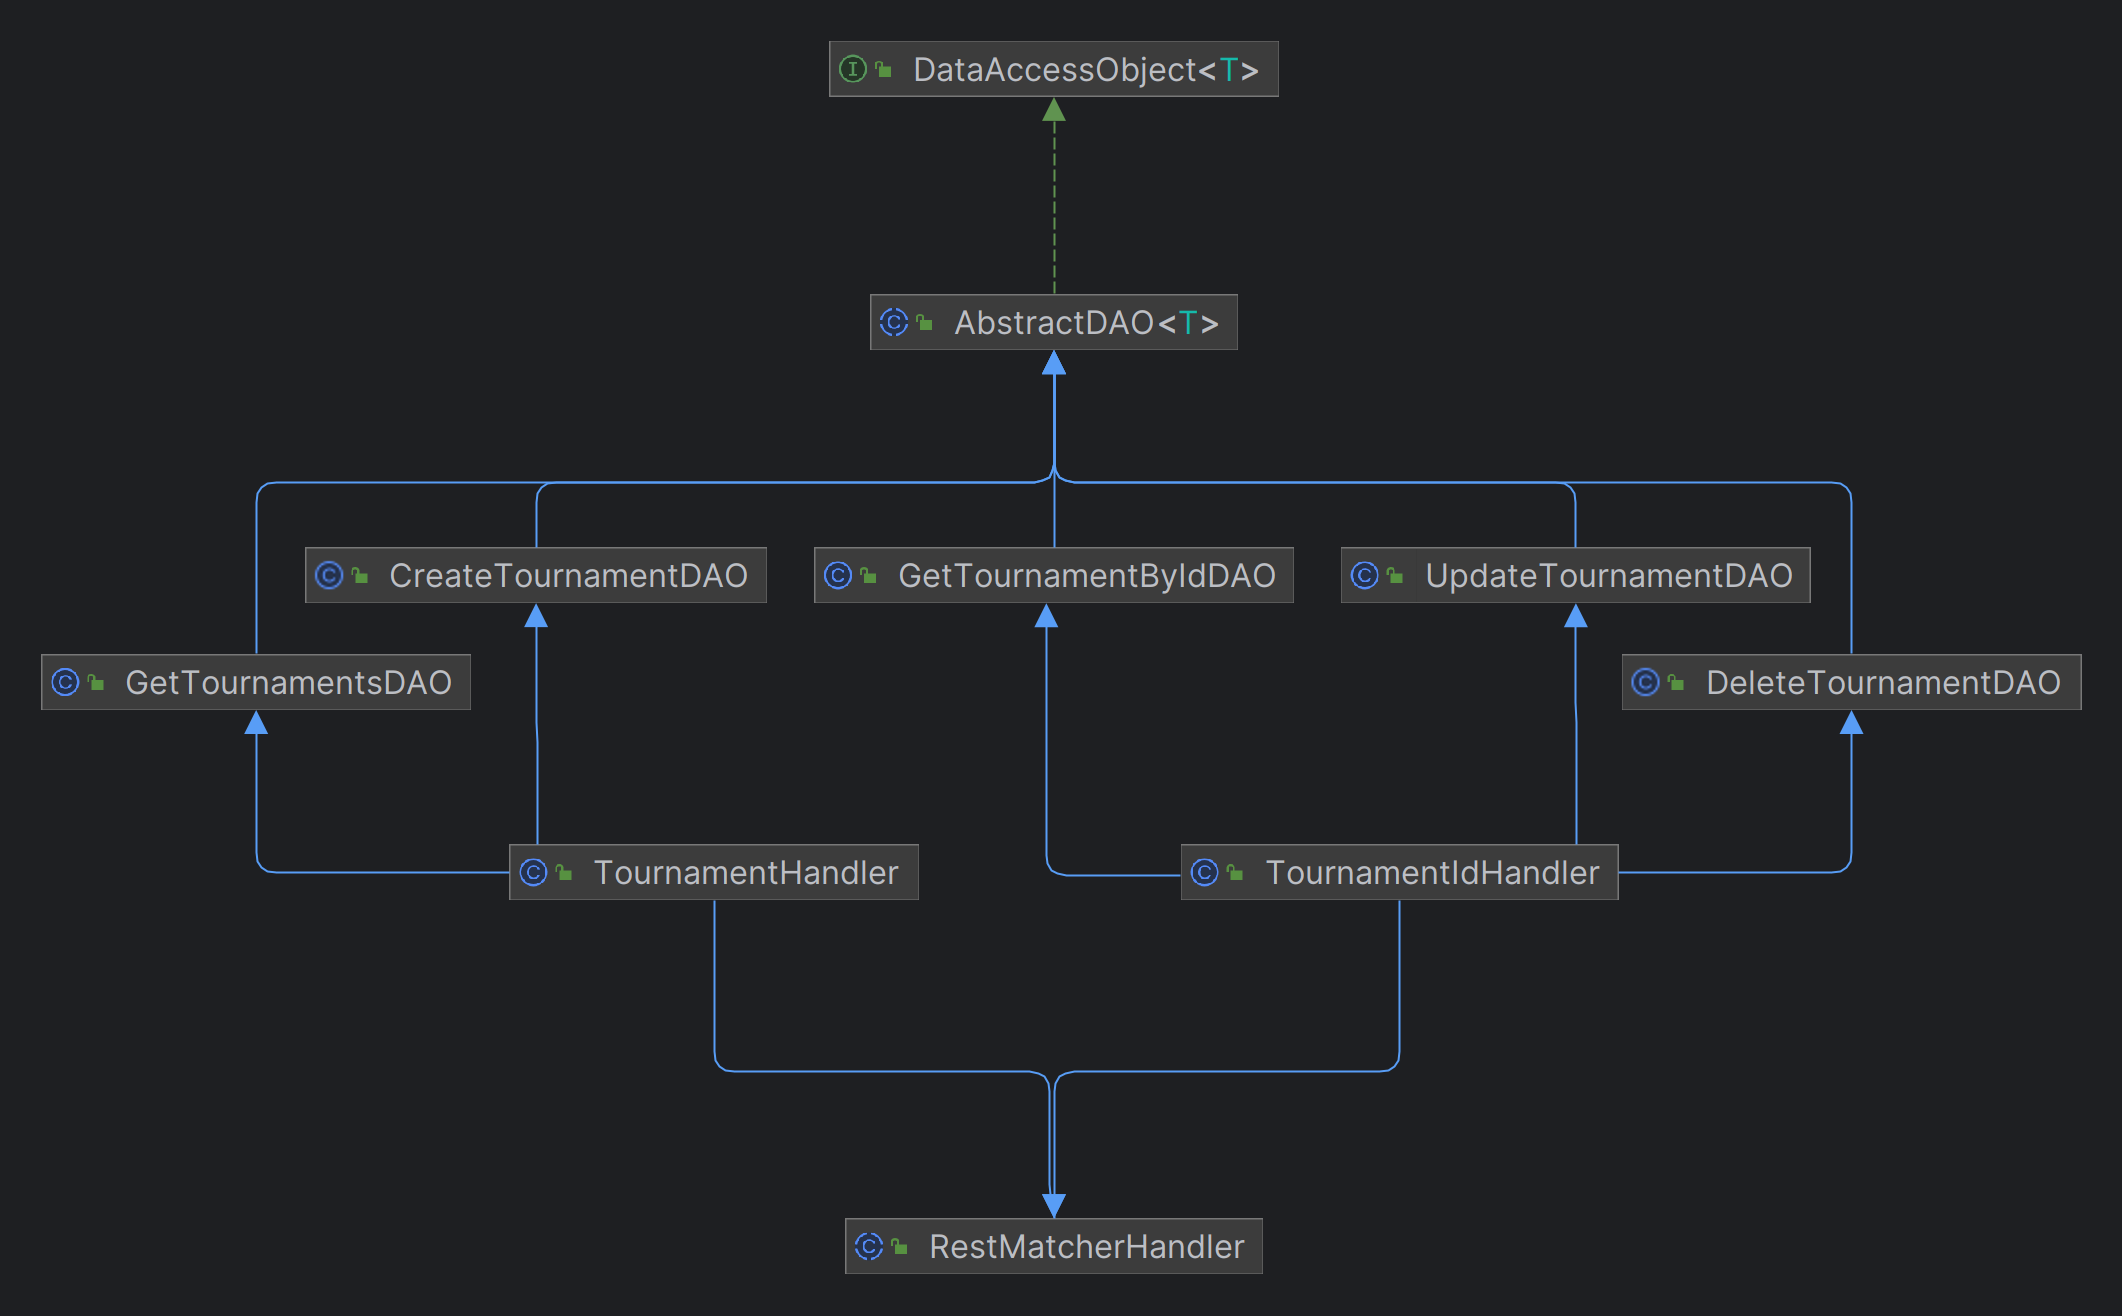
\includegraphics[width = \linewidth]{sections/BLL/ClassDiagram.png}\\\

The image above illustrates a sample of the project's class diagram. We utilize a distinct servlet called \textit{RestMatcherServlet} (not depicted), to manage all the REST endpoints we've established.
Furthermore, servlets were integrated to oversee the non-REST endpoints for each database entity.

Specifically, the image showcases the Java classes responsible for handling the REST endpoints related to tournaments. We employed two distinct handlers, both extending the \textit{RestMatcherHandler}
class, to manage all the tournament's REST endpoints. The \textit{TournamentHandler} handles requests concerning the retrieval of the entire list of active tournaments and the creation of new
ones. Meanwhile, the \textit{TournamentIdHandler} addresses requests related to a single tournament specified by its ID.
Database access is facilitated through specific DAO classes for each type of request. All of these DAOs extend the \textit{AbstractDAO} class, implementing a customized version of the
\textit{doAccess()} method. Similarly, we can handle all the CRUD operations for every entity stored in the database.
